
\begin{figure}[H]
	\centering
	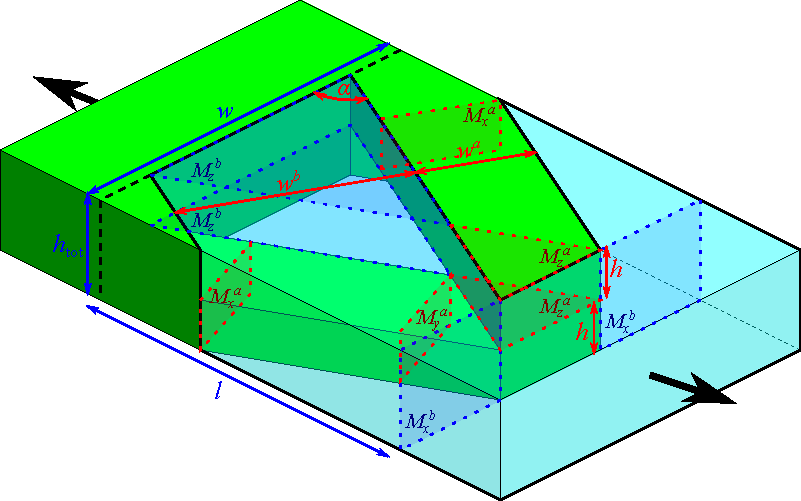
\includegraphics[width=\columnwidth]{sources/method/diagonal_model_v3.pdf}
	\caption{
		One diagonal unit cell connecting material $a$ (left) to material $b$ (right).
		Failure can happen along both the fingers ($M_x$), twice along one finger ($M_y$) or at the interface between the two fingers ($M_z$) for either material.}
	\label{fig:diagonal_model}
\end{figure}



\section{Diagonal Design}

Another option is to place the fingers under an angle as shown in \autoref{fig:diagonal_model}.
There are four design variables: the finger width of both materials: $w^a$ and $w^b$, the length $L$ and the layer thickness $h$.

\section{Failure Modes}
\subsection{Geometry Relations}
From \autoref{fig:diagonal_model}, the following geometry relations can be derived, which are used in the further analysis of the stresses:

\begin{equation}
	\label{eq:tan}
	\tan \alpha = \frac{2L}{w_a + w_b}
\end{equation}

\begin{equation}
	\label{eq:cos}
	\cos \alpha = \frac{w_a + w_b}{\sqrt{ \left( w_a + w_b \right) ^2 + 4L \right)^2 }}
\end{equation}

\begin{equation}
	\label{eq:sin}
	\sin \alpha = \frac{2L}{\sqrt{ \left( w_a + w_b \right) ^2 + 4L \right)^2 }}
\end{equation}


\section{Tension Failure M$_x$}
For the tension failure, we consider the smallest cross sectional area of one finger, which is equal to $w_m \sin \alpha h_m$ . The tensile force perpendicular to this area is equal to $\frac{F}\sin \alpha$, where $F$ is the force per finger. %which was divided by 2 because every finger takes up half of the load. ? - adjust later maybe
This resulted in the following constraint:
\begin{equation}
	\frac{F \sin \alpha}{w_m \sin \alpha h_m} \le \sigma_m
\end{equation}

\begin{equation}
	\frac{F}{w_m  h_m} \le \sigma_{max}
\end{equation}


\section{Shear Failure M$_x$}
The same cross sectional area was taken as above, but now the force that is aligned with this cross section $F \cos \alpha$ was taken to evaluate the shear forces. The maximum shear stress for a rectangular cross sectional area is equal to $\frac{3V}{2A}$. Therefore, the following relation was derived.

\begin{equation}
	\frac{3F \cos \alpha}{h_m w_m \sin \alpha} = \frac{3F }{h_m w_m \tan \alpha} \le \tau_m
\end{equation}

Using \autoref{eq:tan}, the following constraint was the result.
\begin{equation}
	\frac{ 3 F \left(w_a + w_b \right) }{ 4 L w^m h } \le \tau_m	
\end{equation}

\section{Shear Failure M$_z$}
For a triangular cross section, the maximum shear stress is equal to $\frac{3F}{bh}$, where $b$ and $h$ are the base and the height of the triangle respectively. The width is equal to $w_m$, the height is equal to $\frac{w_m}{2} \tan \alpha$. Combining with \autoref{eq:tan}, this resulted in the following constraint.

\begin{equation}
	\frac{ 3 F \left(w_a + w_b \right) }{ w_m ^2 L} \le \tau_m	
\end{equation}


\section{Bending Failure M$_x$}
\todo{Work out derivation}

This resulted in the following constraint for the bending stresses.

\begin{equation}
	\frac{ 3 F \left(w_a + w_b \right) \left(\left(w_a + w_b \right) ^2 + 4L^2 \right)  }{ 2h w_m^2 L^2 }  \le \sigma_m
\end{equation}

\section{Von Mises Stress}
The tensile, shear and bending stresses acting at section $M_x$ were combined into the Von Mises stress criterion.
\todo{Work out derivation and simplify result}

This resulted in the following constraint.
\begin{equation}
	\frac{1}{\sqrt{2}} \sqrt{2 \left( \frac{ F }{ w_m h}   + \frac{ 3 F \left(w_a + w_b \right) \left(\left(w_a + w_b \right) ^2 + 4 L^2 \right)  }{ 2h w_m^2 L^2} \right)^2 + 6 \left(\frac{ 3 F \left(w_a + w_b \right) }{ 4 L w^m h} \right)^2 }		\le 	\sigma_m
	
\end{equation}



The goal is to maximize the strength, while accounting for the failure modes in the constraints.
With that, the optimization problem can be formulated as follows:

\begin{align}
	f: & \max \frac{F}{2h \left(w_a + w_b\right)} \nonumber \\
	\text{subject to:} & \nonumber \\
	g_1: & w_m \ge w_\text{min}^m \\
	g_2: & L_{min} \le L \le L_{max} \\
	g_3: & w_a + w_b \le w_\text{max} \\
	g_4: & \frac{ 3 F \left(w_a + w_b \right) }{ w_m ^2 L} \le \tau_m						&&\text{ Shear failure } M_z^m \\
	g_5:& \frac{1}{\sqrt{2}} \sqrt{2 \left( \frac{ F }{ w_m h}   + \frac{ 3 F \left(w_a + w_b \right) \left(\left(w_a + w_b \right) ^2 + 4 L^2 \right)  }{ 2h w_m^2 L^2} \right)^2 + 6 \left(\frac{ 3 F \left(w_a + w_b \right) }{ 4 L w^m h} \right)^2 }	& 	\le 	\sigma_m	&&\text{ Von Mises criterion } M_x \\
	& \text{for both materials } && m \in \{a, b\} \nonumber 
\end{align}

\iffalse
After reformulation, the equations are as follows:
\begin{align}
	f: \min \frac{2h \left(w_a + w_b\right)}{F } + \alpha \left (w_a + w_b \right ) \\
	\text{subject to:} & \nonumber \\
	g_1: 1 - \frac{w^m}{w_{min}} & \le 0 \\
	g_2: 1 - \frac{L}{L_{min}} & \le 0 \\
		\frac{L}{L_{max}} - 1 & \le 0 \\
	g_3: \frac{w^a + w^b}{w_{max}}  - 1 &\le 0 \\
	g_4: \frac{ 3 F \left(w_a + w_b \right) }{ w^m ^2 L \tau_m} -1 &\le 0							&&\text{ Shear failure } M_z^m \\
	g_5: \frac{1}{\sqrt{2}} \sqrt{2 \left( \frac{ F }{ w^m h}   + \frac{ 3 F \left(w_a + w_b \right) \left(\left(w_a + w_b \right) ^2 + 4 L^2 \right)  }{ 2h w_m^2 L^2} \right)^2 + 6 \left(\frac{ 3 F \left(w_a + w_b \right) }{ 4 L w^m h} \right)^2 }  \sigma_m - 1	& 	\le 	0		&&\text{ Von Mises criterion } M_x^b \\
	& \text{for both materials } && m \in \{a, b\} \nonumber
\end{align}

\fi


